\section{General stuff}

\subsection{Introduction}

The SoundScape Renderer (SSR) is a software framework for real-time spatial
audio reproduction running under GNU/Linux, Mac OS X and possibly some other UNIX
variants.
The current implementation provides Wave Field Synthesis (WFS),
binaural (HRTF-based) reproduction, binaural room (re-)synthesis (BRTF-based
reproduction), head-tracked binaural playback, Ambisonics Amplitude Panning 
(AAP), and Vector Base Amplitude Panning (VBAP).
There are also the slightly exotic Generic Renderer.
For each rendering algorithm there is a separate executable file.
For more details see section~\ref{sec:renderers}.

The SSR is intended as versatile framework for the state-of-the-art
implementation of various spatial audio reproduction techniques. You may use it
for your own academic research, teaching or demonstration activities or whatever
else you like.
However, it would be nice if you would mention the use of the SSR by
e.g.\ referencing~\cite{Geier08:AES} or~\cite{geier2012ssr}.

Note that so far, the SSR only supports two-dimensional reproduction for any
type of renderer. For WFS principally any convex loudspeaker setup
(e.g.\ circles, rectangles) can be used. The loudspeakers should be densely
spaced. For VBAP circular setups are highly recommended. APA does require
circular setups. The binaural renderer can handle only one listener at a time.

\subsection{Quick Start}
\label{sec:quick_start}

After downloading the SSR package, open a shell and use following commands:

\begin{verbatim}
tar xvzf ssr-x.x.x.tar.gz
cd ssr-x.x.x
./configure
make
make install
qjackctl &
ssr my_audio_file.wav
\end{verbatim}

You have to replace \texttt{x.x.x} with the current version number, e.g.\
\texttt{0.4.0}.
With above commands you are performing the following steps:
\begin{itemize}
  \item Unpack the downloaded tarball containing the source-code.
  \item Go to the extracted directory%
    \footnote{Note that most relative paths which are
    mentioned in this document are relative to this folder,
    which is the folder where the SSR tarball was extracted. Therefore,
    e.g.\ the \texttt{src/} directory could be something like
    \texttt{\$HOME/ssr-x.x.x/src/} where ``x'' stands for the 
    version numbers.}.
  \item Configure the SSR.
  \item Install the SSR.
  \item Open the graphical user interface for JACK (\verb+qjackctl+).
    Please click ``Start'' to start the server.
    As alternative you can start JACK with
    \begin{quote}
    \texttt{jackd -d alsa -r 44100}
    \end{quote}
    See section~\ref{sec:running_ssr} and
    \texttt{man jackd} for further options.
  \item Open the SSR with an audio file of your choice. This can be a
    multichannel file.
\end{itemize}
%
This will load the audio file \texttt{my\_audio\_file.wav} and create a virtual
sound source for each channel in the audio file.
By default, the SSR will start with the binaural renderer. Please use headphones
to listen to the generated output!

If you don't need a graphical user interface and you want to dedicate all your
resources to audio processing, try
\begin{quote}
\texttt{ssr --no-gui my\_audio\_file.wav}
\end{quote}
%
For further options, see section~\ref{sec:running_ssr} and \texttt{ssr --help}.

\subsection{Audio Scenes}
\label{sec:audio_scenes}

\subsubsection{Format}

The SSR can open \texttt{.asd} files (refer to section \ref{sec:asdf}) as well
as normal audio files. If an audio file is opened, SSR creates an individual
virtual sound source for each channel which the audio file contains. If a
two-channel audio file is opened, the resulting virtual sound sources are
positioned like a virtual stereo loudspeaker setup with respect to the location
of the reference point. For audio files with more (or less) channels, SSR randomly
arranges the resulting virtual sound sources.
All types that
ecasound and libsndfile can open can be used. In particular this includes \texttt{.wav}, \texttt{.aiff}, \texttt{.flac} and \texttt{.ogg} files.

In the case of a scene being loaded from an \texttt{.asd} file, all audio files
which are associated to virtual sound sources are replayed in parallel and
replaying starts at the beginning of the scene. So far, a dynamic handling of
audio files has not been implemented.

\subsubsection{Coordinate System}

\begin{figure}
\psfrag{alpha}{$\alpha$} \psfrag{r}{$r$} \psfrag{x}{$x$}
\psfrag{y}{$y$} \psfrag{bx}{${\bf x}$}
\psfrag{alphaprime}{$\alpha'$}\psfrag{yprime}{$y'$} \psfrag{xprime}{$x'$}
\begin{center}
\subfigure[\label{fig:global_coordinate_system}{Global coordinate system.}]
{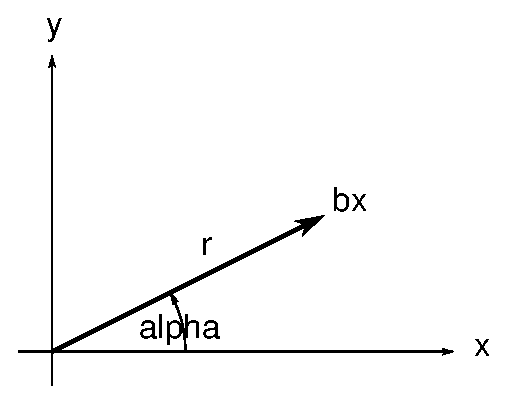
\includegraphics[width=.45\linewidth]{images/coordinate_system.eps}} \hfill
\subfigure[\label{fig:local_coordinate_system}{Local coordinate system relative
to the reference. The latter is indicated by the rhomb.}]
{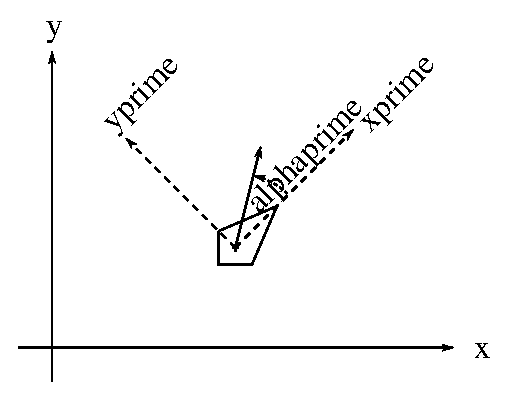
\includegraphics[width=.45\linewidth]{images/local_coordinate_system.eps}}
\caption{\label{fig:coordinate_system}{The coordinate system used in the SSR.
In ASDF $\alpha$ and $\alpha'$ are referred to as azimuth (refer to section
\ref{sec:asdf}).}}
\end{center}
\end{figure}

Fig.~\ref{fig:global_coordinate_system} depicts the global coordinate system
used in the SSR. Virtual sound sources as well as the reference are positioned
and orientated with respect to this coordinate system. For loudspeakers,
positioning is a bit more tricky since it is done with respect to a local
coordinate system determined by the reference. Refer to 
Fig.~\ref{fig:local_coordinate_system}. The loudspeakers are positioned with 
respect to the primed coordinates ($x'$, $y'$, etc.).

The motivation to do it like this is to have a means to virtually move the
entire loudspeaker setup inside a scene by simply moving the reference. This
enables arbitrary movement of the listener in a scene independent of the
physical setup of the reproduction system.

Please do not confuse the origin of the coordinate system with the reference. 
The coordinate system is static and specifies absolute positions.

The reference is movable and is always taken with respect to the current 
reproduction setup. The loudspeaker-based methods do not
consider the orientation of the reference point but its location influences the
way loudspeakers are driven. E.g., the reference location corresponds to the
\emph{sweet spot} in VBAP. It is therefore advisable to put the reference point
to your preferred listening position. In the binaural methods
the reference point represents the listener and indicates the position and 
orientation of the latter. It is therefore essential to set it properly in this
case.

Note that the reference position and orientation can of course be updated in
real-time. For the loudspeaker-based methods this is only useful to a limited
extent unless you want to move inside the scene. However, for the binaural 
methods it is essential that both the reference position and orientation 
(i.e.\ the listener's position and orientation) are tracked and updated in 
real-time. Refer also to Sec.~\ref{sec:head_tracking}.

\subsection{Audio Scene Description Format (ASDF)}
\label{sec:asdf}

Besides pure audio files, SSR can also read the current development version of
the \emph{Audio Scene Description Format
(ASDF)}~\cite{Geier08:DAGA}. Note however that so
far, we have only implemented descriptions of static features. That
means in the current state it is not possible to describe
e.g.~movements of a virtual sound source. As
you can see in the example audio scene below, an audio file can be
assigned to each virtual sound source. The replay of all involved
audio files is synchronized to the replay of the entire scene. That
means all audio files start at the beginning of the sound scene. If
you fast forward or rewind the scene, all audio files fast forward
or rewind. {\bf Note that it is sigificantly more efficient to read data from
an interleaved multichannel file compared to reading all channels from
individual files}.

\subsubsection{Syntax}

The format syntax is quite self-explanatory. See the examples below.
Note that the paths to the audio files can be either absolute (not
recommended) or relative to the directory where the scene file is
stored. The exact format description of the ASDF can be found in the
XML Schema file \texttt{asdf.xsd}.

\noindent Find below a sample scene description:

\begin{verbatim}
<?xml version="1.0"?>
<asdf version="0.1">
  <header>
    <name>Simple Example Scene</name>
  </header>
  <scene_setup>
    <source name="Vocals" model="point">
      <file>audio/demo.wav</file>
      <position x="-2" y="2"/>
    </source>
    <source name="Ambience" model="plane">
      <file channel="2">audio/demo.wav</file>
      <position x="2" y="2"/>
    </source>
  </scene_setup>
</asdf>
\end{verbatim}

\noindent The input channels of a soundcard can be used by specifying the
channel number instead of an audio file, e.g. \verb|<port>3</port>| instead of
\verb|<file>my_audio.wav</file>|.

\subsubsection{Examples}

We provide an audio scene example in ASDF with this release. You find it in
\texttt{data/scenes/live\_input.asd}. If you load this file into the SSR it
will create 4 sound sources which will be connected to the first four channels
of your sound card. If your sound card happens to have less than four outputs, less sources will be created accordingly.
More examples for audio scenes can be downloaded from the SSR
website~\cite{ssr}.

\subsection{IP Interface}

\label{sec:ip_interface}

One of the key features of the SSR is an interface which lets you
remotely control the SSR via a TCP socket using XML messages. This
interface enables you to straightforwardly connect any type of
interaction tool from any type of operating system.
The format of the messages sent over the network is still under development and
may very likely change in future versions.
Please find some
brief information in section~\ref{sec:network}.

%An example how the SSR can be controlled via its network interface is the
%Python client located in the directory \verb|python_client/| and the provided
%Pure Data patches.

\subsection{Bug Reports, Feature Requests and Comments}

%For a list of known problems have a look at the SSR development website%
%\footnote{\url{https://dev.qu.tu-berlin.de/projects/ssr/wiki/Known_Issues}}.
Please report any bugs, feature requests and comments to
\contactadress. We will keep track of them and will try to fix them
in a reasonable time. The more bugs you report the more we can fix.
Of course, you are welcome to provide bug fixes.~\smiley

\subsection{Contributors}

\IfFileExists{authors.tex}{\input{authors}}{%
For a list of contributors, please see the file \texttt{AUTHORS}.}

\subsection{Your Own Contributions}

The SSR is thought to provide a state of the art implementation of
various spatial audio reproduction techniques. We therefore would
like to encourage you to contribute to this project since we can
not assure to be at the state of the art at all times ourselves.
Everybody is welcome to contribute to the development of the SSR.
However, if you are planning to do so, we kindly ask you to contact
us beforehand (e.g.~via \contactadress). The SSR is in a rather
temporary state and we might apply some changes to its architecture.
We would like to ensure that your own implementations stay compatible
with future versions.

\begin{comment}
\subsection{Version history}

\begin{itemize}
\item Initial release: 0.1
\end{itemize}
\end{comment}
